\begin{figure}[t]
    \centering
    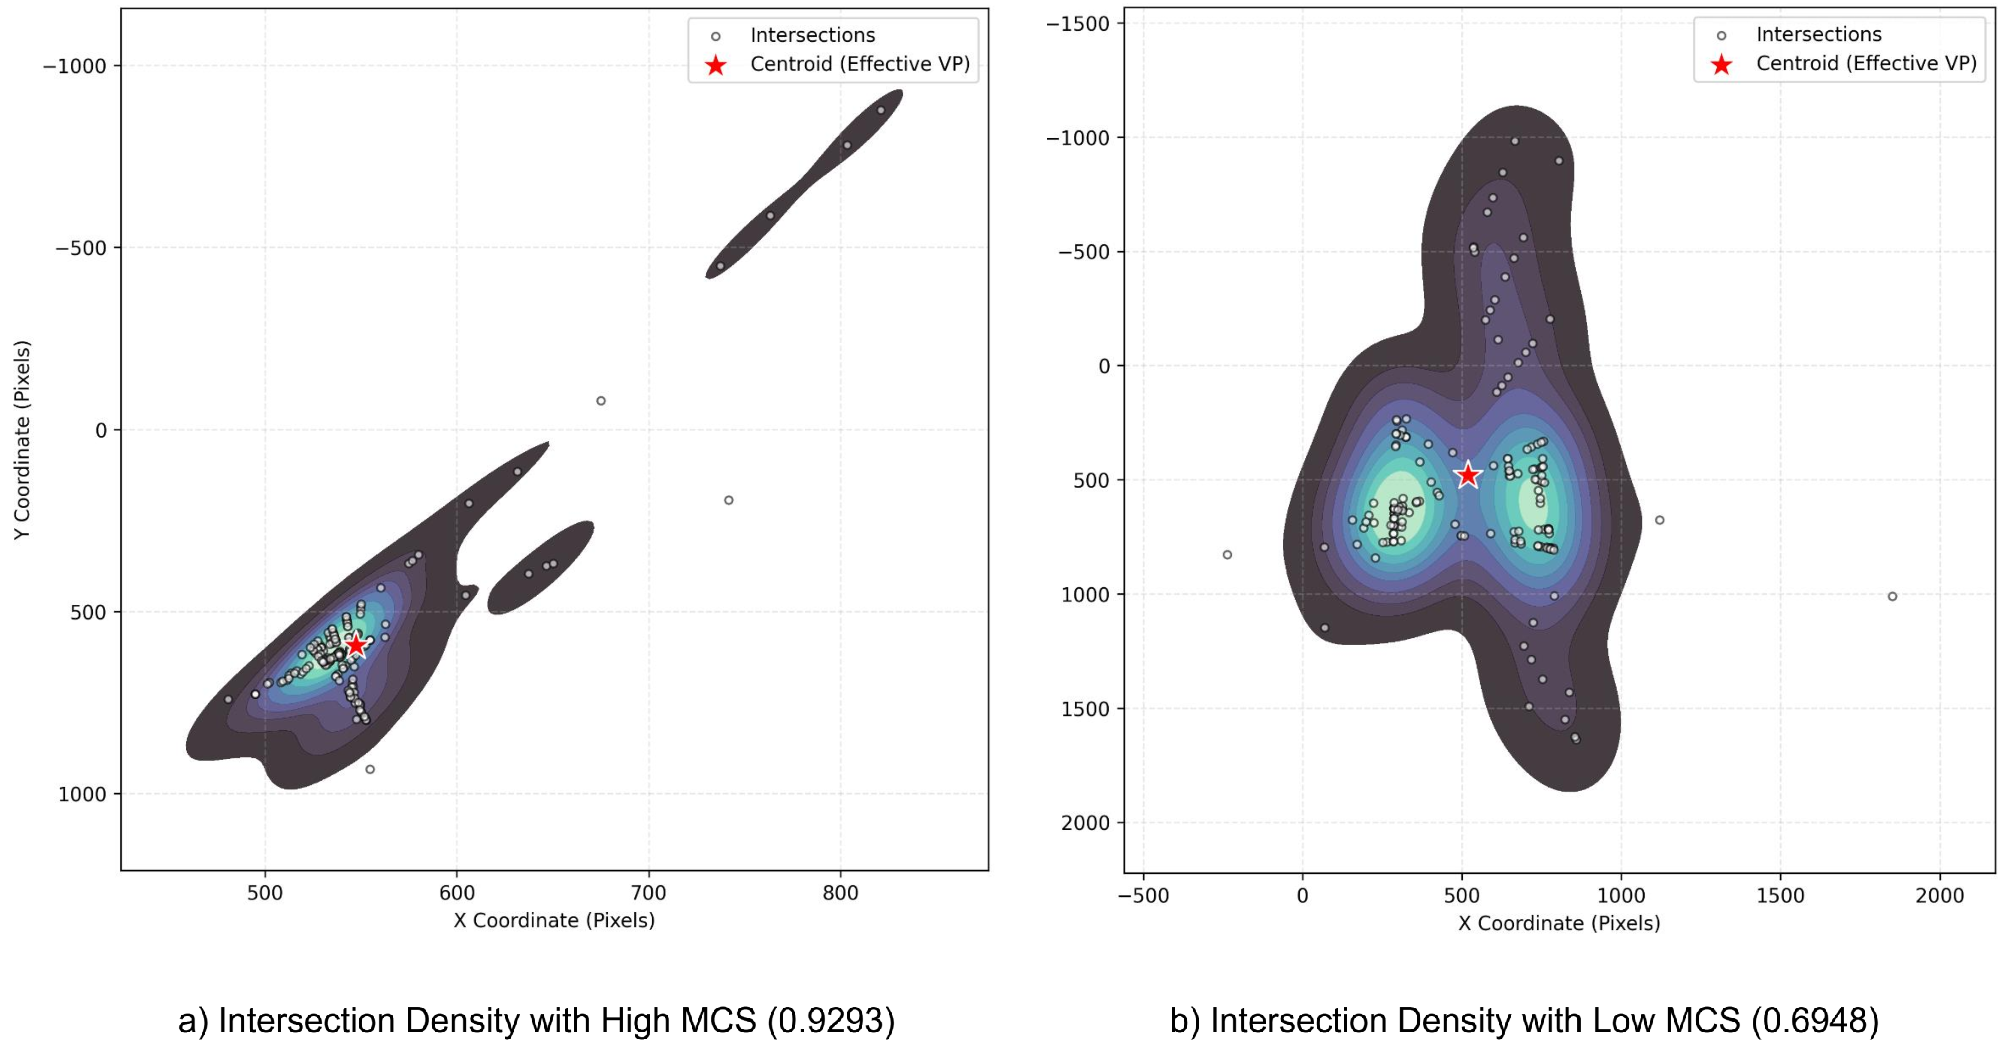
\includegraphics[width=\linewidth]{figures/MCSVisualization.pdf}
    \vspace{-5mm}
    \caption{Visualization of the Mirror Consistency Score (MCS). (Left) A physically correct reflection yields tightly clustered intersection points around the vanishing point, resulting in a high MCS. (Right) Perspective mismatches cause the intersection points to scatter, which is penalized with a low score.}
    \label{fig:mcs_visualization}
\end{figure}